\documentclass{beamer}
\usepackage[latin1]{inputenc}
\usepackage{times}
\usepackage{tikz}
\usetheme{Luebeck}
%\usecolortheme{albatross}
\usepackage{amsmath,amsfonts,amsthm,amssymb}
\usepackage{setspace}
\usepackage{Tabbing}
\usepackage{fancyhdr}
\usepackage{lastpage}
\usepackage{extramarks}
\usepackage{chngpage}
\usepackage{soul,color}
\usepackage{graphicx,float,wrapfig}
\usepackage{xcolor}
\usepackage{listings}
\usepackage{float}
%\usepackage{subfloat}
\usepackage{subfigure}
\usepackage{caption}
\usepackage{enumitem}
\usepackage{algpseudocode}

\definecolor{darkorange}{RGB}{240, 120, 0}
\definecolor{darkgreen}{RGB}{0, 128, 0}
\definecolor{darkred}{RGB}{128, 0, 0}

\setbeamercolor{background canvas}{bg=white}
\setbeamercolor{frametitle}{fg=white, bg=darkorange}
\setbeamercolor{normal text}{bg=black,fg=black}
\setbeamercolor{structure}{bg=black, fg=darkorange}


\lstdefinestyle{customc}{
  belowcaptionskip=1\baselineskip,
  breaklines=true,
  frame=L,
  xleftmargin=\parindent,
  language=Python,
  showstringspaces=false,
  basicstyle=\footnotesize\ttfamily,
  keywordstyle=\bfseries\color{green!40!black},
  commentstyle=\itshape\color{purple!40!black},
  identifierstyle=\color{blue},
  stringstyle=\color{orange},
}

\lstdefinestyle{customc}{
  belowcaptionskip=1\baselineskip,
  breaklines=true,
  frame=L,
  xleftmargin=\parindent,
  language=Python,
  showstringspaces=false,
  basicstyle=\footnotesize\ttfamily,
  keywordstyle=\bfseries\color{green!40!black},
  commentstyle=\itshape\color{purple!40!black},
  identifierstyle=\color{blue},
  stringstyle=\color{orange},
}

\lstdefinestyle{customcsmall}{
  belowcaptionskip=1\baselineskip,
  breaklines=true,
  frame=L,
  xleftmargin=\parindent,
  language=Python,
  showstringspaces=false,
  basicstyle=\footnotesize\ttfamily,
  keywordstyle=\bfseries\color{green!24!black},
  commentstyle=\itshape\color{purple!24!black},
  identifierstyle=\color{blue},
  stringstyle=\color{orange},
}

\lstdefinestyle{customcsmall}{
  belowcaptionskip=1\baselineskip,
  breaklines=true,
  frame=L,
  xleftmargin=\parindent,
  language=Python,
  showstringspaces=false,
  basicstyle=\footnotesize\ttfamily,
  keywordstyle=\bfseries\color{green!24!black},
  commentstyle=\itshape\color{purple!24!black},
  identifierstyle=\color{blue},
  stringstyle=\color{orange},
}

\definecolor{MidGreen}{HTML}{00AA00}
\definecolor{MidYellow}{HTML}{AAAA00}

\title{Lecture 28: Last Lecture!}
\date{4/26/2016}
\institute{Chris Tralie, Duke University}
\author{COMPSCI/MATH 290-04}
\begin{document}

\frame{\titlepage}

\begin{frame}{Announcements}
\begin{itemize}[label=$\vartriangleright$]

\item Group Assignment 3 Final Deadline Tonight

\item Last office hours this Thursday

\item Final Project Videos due \textcolor{red}{Sunday 5/1}

\item Final Project Feedback due Monday 5/2

\item Final Project Deliverables due Tuesday 5/3

\item Grades coming in soon!

\end{itemize}

\end{frame}


\begin{frame}{Table of Contents}

\begin{itemize}[label=$\blacktriangleright$]
	\item Raffle!
\end{itemize}

\begin{itemize}[label=$\vartriangleright$]
	\item My Teaching Philosophy / Course In Review
\end{itemize}


\begin{itemize}[label=$\vartriangleright$]
	\item Advice / Post-Course Homework
\end{itemize}

\end{frame}



\begin{frame}{Cotangent Weights: Voronoi Area Interpretation}

\begin{figure}[t]
    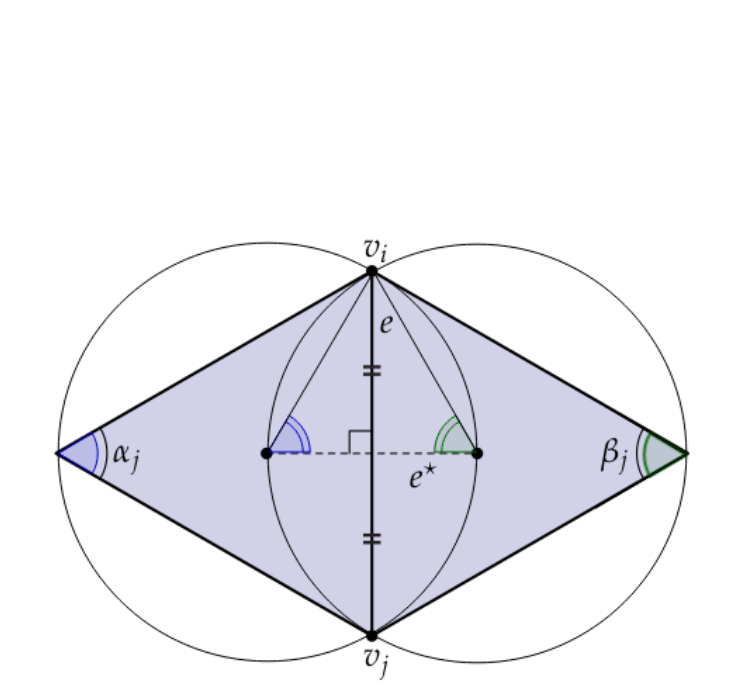
\includegraphics[width=0.7\textwidth]{CotWeights.png}
\end{figure}

\end{frame}


\begin{frame}{Raffle}

First Item: 3D Scan of Head, 6 draws

\end{frame}

\begin{frame}{Raffle}

Second Item: 3D Printed Head, 3 Draws

\end{frame}


\begin{frame}{Table of Contents}

\begin{itemize}[label=$\vartriangleright$]
	\item Raffle!
\end{itemize}

\begin{itemize}[label=$\blacktriangleright$]
	\item My Teaching Philosophy / Course In Review
\end{itemize}


\begin{itemize}[label=$\vartriangleright$]
	\item Advice / Post-Course Homework
\end{itemize}

\end{frame}


\begin{frame}{What The Heck Was This Course??}

\begin{itemize}[label=$\vartriangleright$]
\item \textcolor{blue}{Computer Graphics} - \textcolor{red}{Rendering} - \textcolor{red}{Image Processing} + \textcolor{MidGreen}{Geometry} + \textcolor{MidGreen}{Data Analytics} + \textcolor{MidGreen}{Signal Processing}
\end{itemize}

\uncover<2->{
\begin{itemize}[label=$\vartriangleright$]

\item 200-level course!  Focus on {\em fundmentals}

\end{itemize}
}

\uncover<3->{
\begin{itemize}[label=$\vartriangleright$]

\item Practical skills and applications (Javascript/Python/Numerical Coding)...

\end{itemize}
}

\uncover<4->{
\begin{itemize}[label=$\vartriangleright$]

\item ...but also {\em straight up math} in a visual way

\end{itemize}
}

\uncover<5->{

\begin{itemize}[label=$\vartriangleright$]

\item Meant to take everyone out of their comfort zones

\end{itemize}

}

\end{frame}

\begin{frame}{Setting the Bar High...}

...but largely keeping that a secret

\begin{figure}[t]
    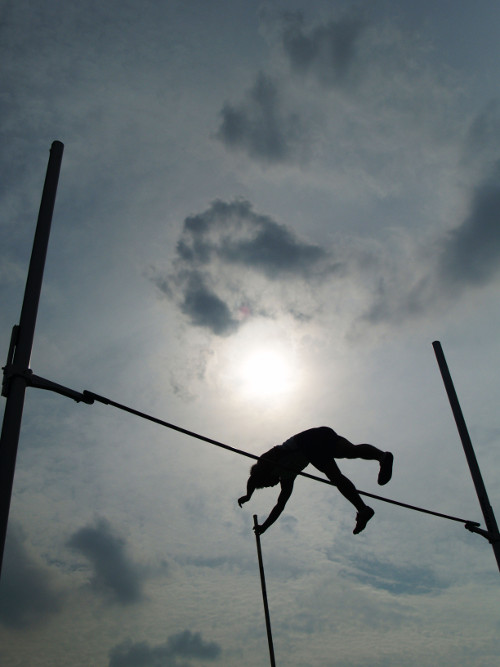
\includegraphics[width=0.5\textwidth]{PoleVault.jpg}
\end{figure}

\end{frame}

\begin{frame}{Overcoming Math Fear}

\begin{figure}[t]
    
\includegraphics[width=0.5\textwidth]{math-anxiety.jpg}
\end{figure}

\tiny \textcolor{red}{http://www.kids-activities-learning-games.com/images/math-anxiety.jpg}

\small
Most common fear in beginning of class survey, but {\em everyone} stepped it up.  Congratulations!!!

\end{frame}

\begin{frame}{Art Contests}

Own your work, {\em be creative!}

\end{frame}


\begin{frame}{Skeleton Code}

\begin{figure}[t]
    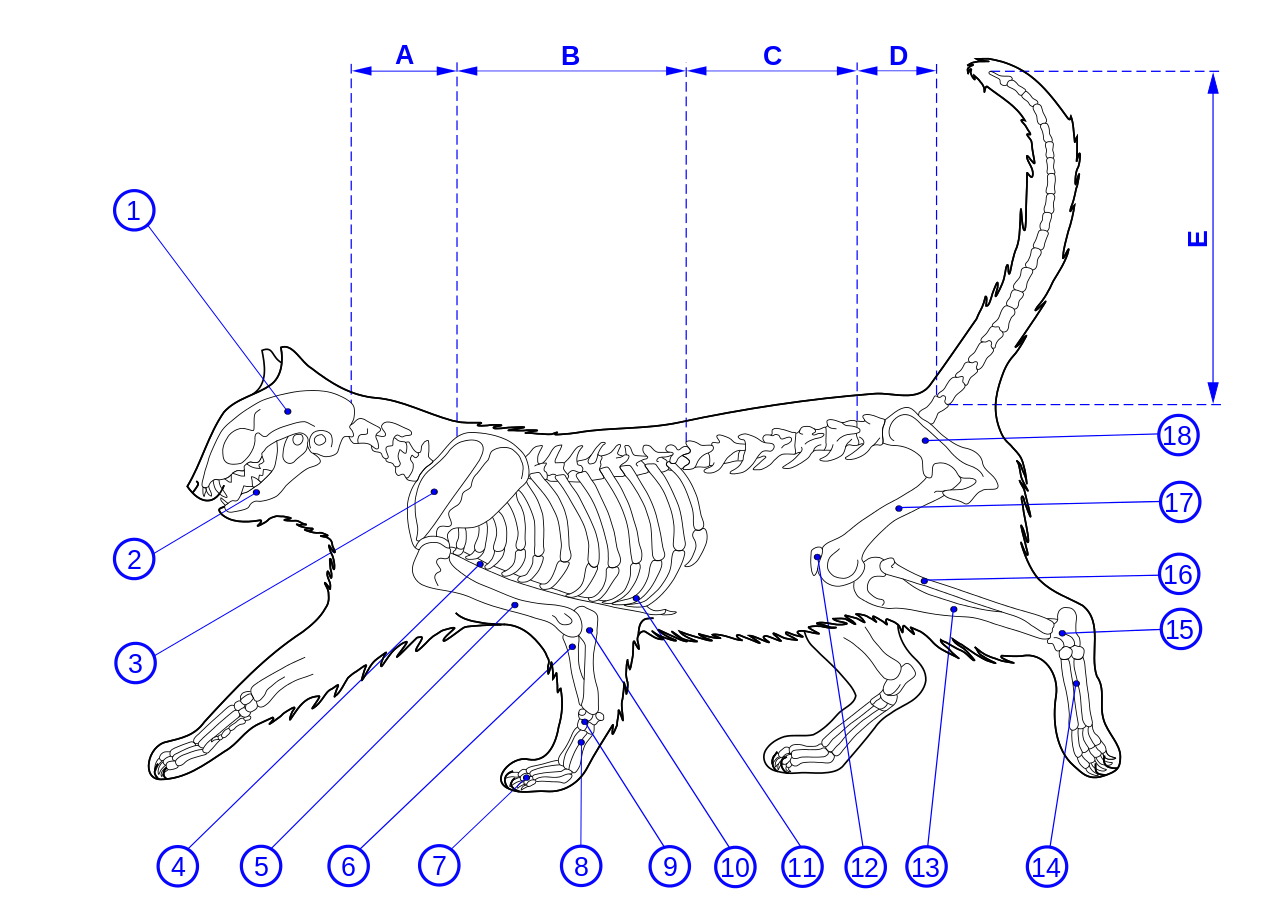
\includegraphics[width=0.8\textwidth]{catskeleton.png}
\end{figure}

Use the code in your own future projects!!  It's all open source

\end{frame}



\begin{frame}{Look At What You've Learned!}

\begin{figure}[t]
    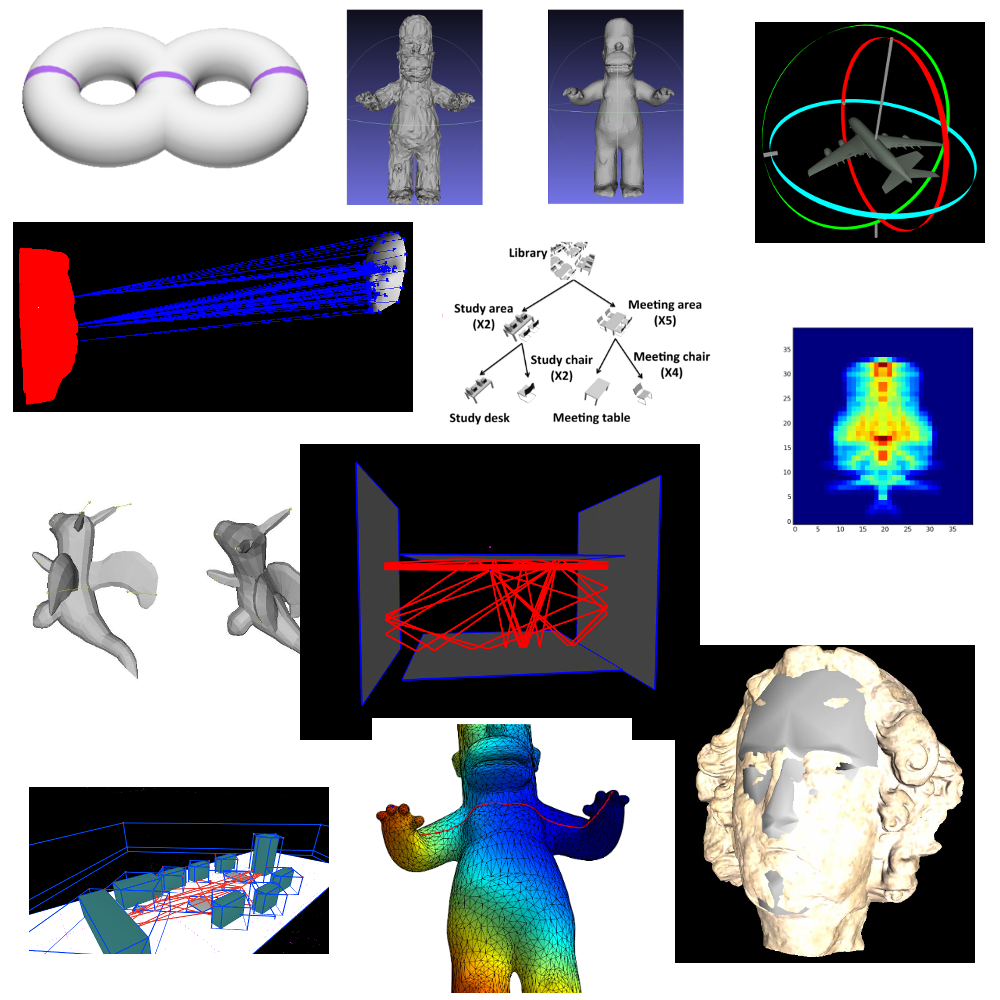
\includegraphics[width=0.7\textwidth]{CourseInReview.png}
\end{figure}


\end{frame}

\begin{frame}{Table of Contents}

\begin{itemize}[label=$\vartriangleright$]
	\item Raffle!
\end{itemize}

\begin{itemize}[label=$\vartriangleright$]
	\item My Teaching Philosophy / Course In Review
\end{itemize}


\begin{itemize}[label=$\blacktriangleright$]
	\item Advice / Post-Course Homework
\end{itemize}

\end{frame}


\begin{frame}{``I Don't Know Anything''?!!...}

...good!  Keep going!

\uncover<2->{
Learning is a lifelong thing, things come into focus slowly over time
}

\end{frame}


\begin{frame}{Geniuses?!}

{\em This class was a ``no genius zone''}.  Everyone is capable

\begin{figure}[t]
    
\includegraphics[width=0.5\textwidth]{genius.png}
\end{figure}

It's about working hard, challenging yourself, {\em struggling}, and growing

\end{frame}

\begin{frame}{Nobody Is Special...}

...but as a result, {\em everyone} is special!  I really enjoyed getting to know you all

\end{frame}

\begin{frame}{Two Secrets}

1. I don't know everything (maybe that wasn't such a secret...).  This was important so you also weren't afraid to make mistakes and admit you didn't know something!

\uncover<2->{
2.   You guys are so good, that I was really just your coach

\begin{figure}[t]
    
\includegraphics[width=0.5\textwidth]{coach.jpg}
\end{figure}

}

\end{frame}

\begin{frame}{Authenticity}

\begin{figure}[t]
    
\includegraphics[width=0.5\textwidth]{keepitreal.png}
\end{figure}

Get to know yourself and your values

\end{frame}


\begin{frame}{Liberal Arts}
\textcolor{red}{Be a patron and protector of the liberal arts!}

\begin{figure}[t]
    
\includegraphics[width=\textwidth]{Einstein_LiberalArts.jpg}
\end{figure}


There is a war being waged right now against the liberal arts.  Pick the correct side.  You have the power

\end{frame}

\begin{frame}{Stereotype Threat}

\begin{figure}[t]
    
\includegraphics[width=0.35\textwidth]{WhistlingVivaldi.jpg}
\end{figure}

\small This is a real thing, and it's been scientifically proven again and again.  Be aware of it.  Work to foster positive and inclusive environments

\end{frame}

\begin{frame}{Thank you!!!}

Teaching was my dream.  You made my dreams come true this semester.  Stay in touch!

\begin{figure}[t]
    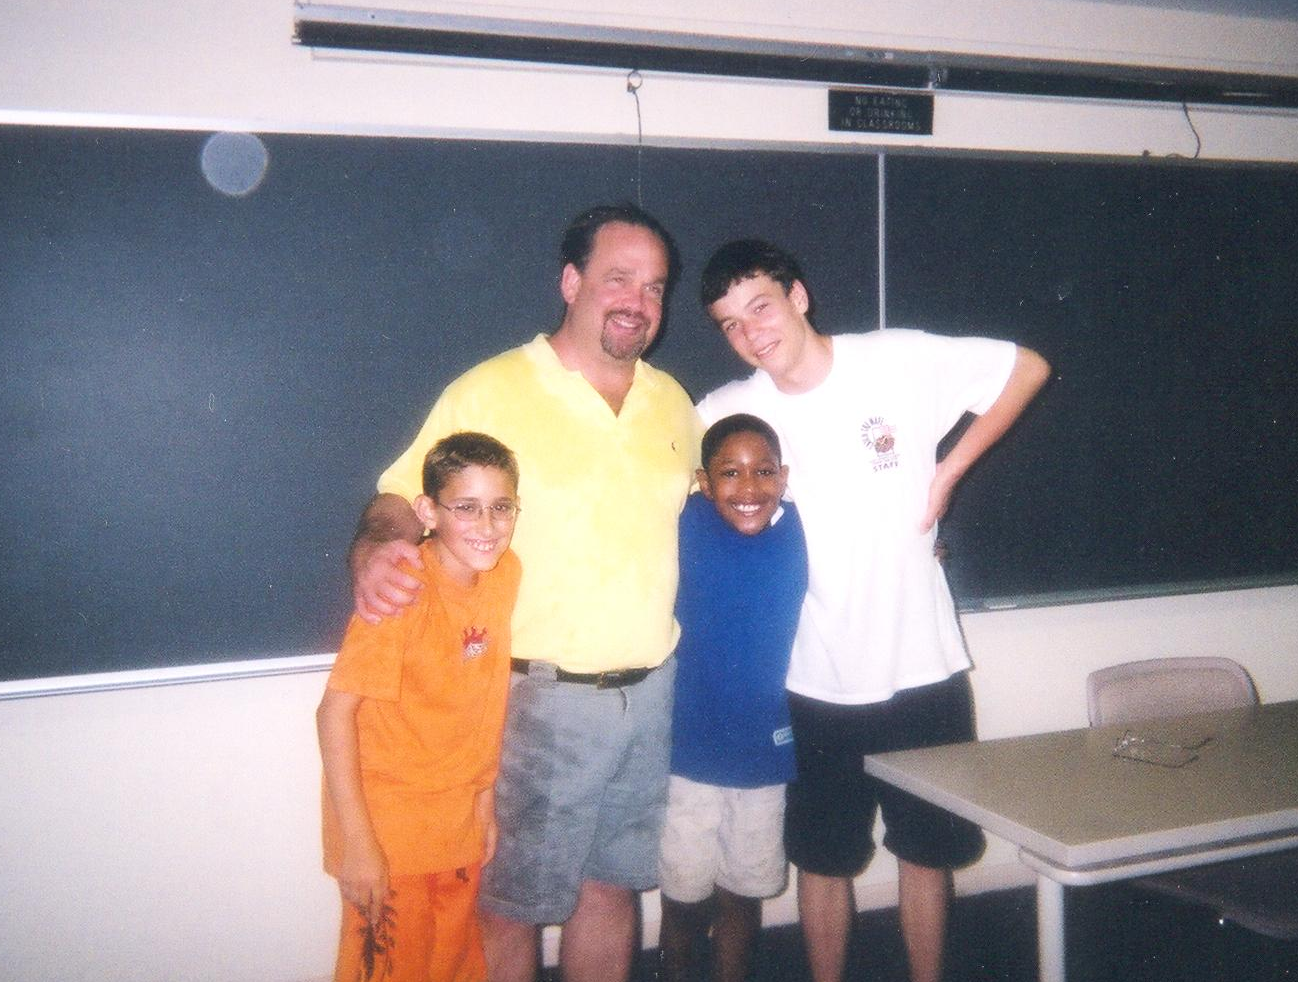
\includegraphics[width=0.7\textwidth]{christeaching.png}
\end{figure}
\tiny Temple University Ambler Summer 2003, ``Fun with Math, Science, And Computers''

\end{frame}

\end{document}

